\documentclass[tikz,border=5pt]{standalone}
\usepackage{tikz}
\usetikzlibrary{arrows.meta}
\usepackage{amsmath}
\usepackage{physics}

\ExplSyntaxOn
\msg_redirect_name:nnn { siunitx } { physics-pkg } { none }
\ExplSyntaxOff

\begin{document}

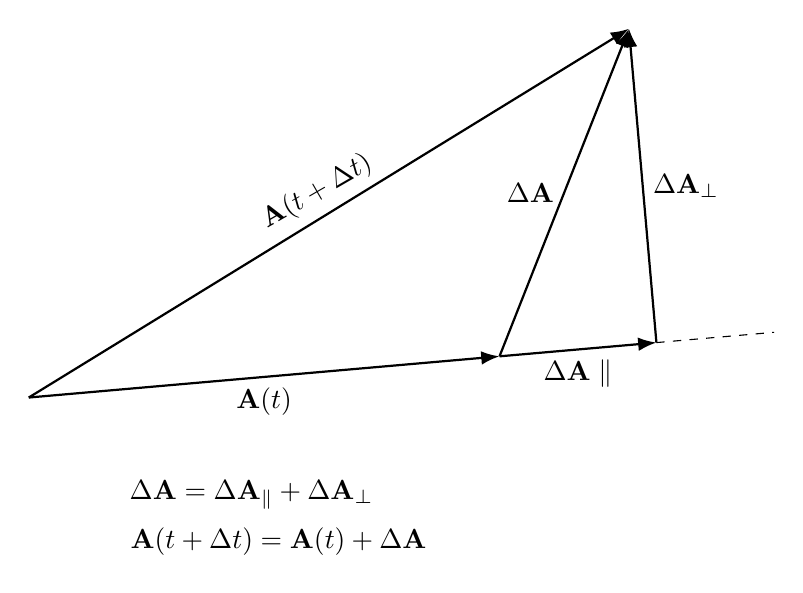
\begin{tikzpicture}[scale=2, rotate=5]
    \coordinate (A) at (3, 0);
    \coordinate (B) at (4, 0);
    \coordinate (C) at (4, 2);

    \draw[-{Latex}, thick] (0, 0) -- (A) node [midway, below] {$\vb{A} (t)$};
    \draw[-{Latex}, thick] (A) -- (B) node [midway, below] {$\Delta \vb{A} \parallel$};
    \draw [dashed] (B)-- ++(0.75, 0);

    \draw[-{Latex}, thick] (0, 0) -- (C) node [midway, above, rotate=30] {$\vb{A} (t + \Delta t)$};
    \draw[-{Latex}, thick] (A) -- (C) node [midway, left] {$\Delta \vb{A}$};
    \draw[-{Latex}, thick] (B) -- (C) node [midway, right] {$\Delta \vb{A}_{\perp}$};

    \node at (1.5, -0.75) () {\hspace*{-0.7cm} $\Delta \vb{A} = \Delta \vb{A}_{\parallel} + \Delta \vb{A}_{\perp}$};
    \node at (1.5, -1.05) () {$\vb{A} (t + \Delta t) = \vb{A} (t) + \Delta \vb{A}$};

\end{tikzpicture}

\end{document}
